% !TeX root = ../main.tex
\section{Reduktion des Netzwerks}
\label{sec:reduktion}

Die Athletenprojektion ist mit über 1,2 Millionen Kanten für viele Verfahren
und Darstellungen zu gross. Wir reduzieren sie zuerst über das Kantengewicht.
Anschliessend betrachten wir das Ergebnis getrennt nach Geschlecht (Local
View), zusammengefasst nach Profilnation (Global View), kombiniert am
Beispiel der Schweiz (Contextual View) und aus der Sicht eines einzelnen
Athleten (Ego-Netzwerk).

\subsection{Filtern nach Kantengewicht}
Die Gewichte sind stark rechtsschief (Abbildung~\ref{fig:kantengewichte}A).
71,0\,\% der Kanten beruhen auf nur einem gemeinsamen Veranstaltungstag. Der
Median beträgt 1, das 99.~Perzentil 6 und das Maximum 25.
Abbildung~\ref{fig:kantengewichte}B zeigt die Wirkung verschiedener
Mindestgewichte. Alle 13\,156 Athleten bleiben dabei als Knoten erhalten.

\begin{figure}[H]
  \centering
  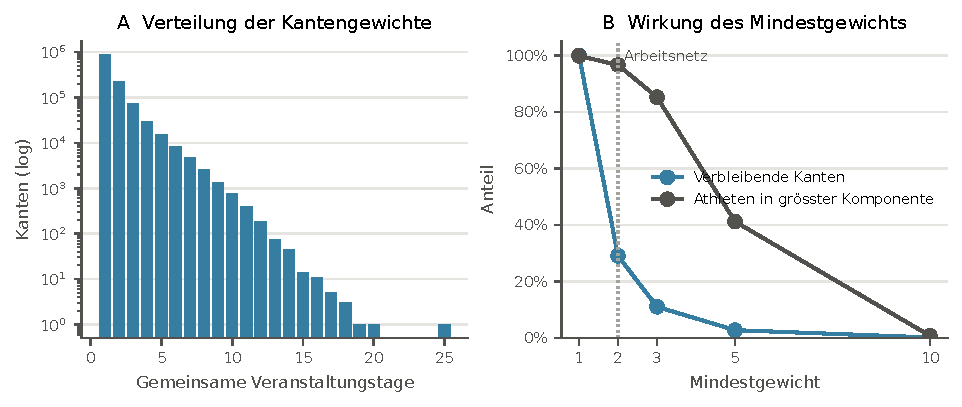
\includegraphics[width=\textwidth]{04_kantengewichte.pdf}
  \caption{Kantengewichte der Athletenprojektion. A: Anzahl Kanten je
  Zahl gemeinsamer Tage (logarithmische Achse). B: Anteil verbleibender
  Kanten (blau) und Anteil der Athleten in der Giant Component (grau) je
  Mindestgewicht, gepunktet das Arbeitsnetz. Eigene Auswertung.}
  \label{fig:kantengewichte}
\end{figure}

Als Arbeitsnetz verwenden wir ein Mindestgewicht von zwei gemeinsamen Tagen.
Es entfernt 71\,\% der Kanten, die Giant Component, also die grösste
zusammenhängende Komponente, umfasst aber weiterhin 96,6\,\% der Athleten. Die Zahl isolierter Athleten steigt
dabei von 20 auf 413. Ab Gewicht 5 liegt mehr als die Hälfte der Athleten
ausserhalb der Giant Component. Gewicht 3 dient nur der Darstellung in
Abbildung~\ref{fig:athletenprojektion}. Die Giant Component des
Arbeitsnetzes mit 12\,709 Athleten verwenden wir nur für Verfahren, die
einen zusammenhängenden Graphen voraussetzen. Der Filter bevorzugt Athleten,
deren Bestleistungen wiederholt an denselben Veranstaltungen erfasst sind.
Spätere Ergebnisse hängen deshalb auch vom gewählten Schwellenwert ab.

\subsection{Local View nach Geschlecht}
Tabelle~\ref{tab:local} vergleicht die Teilnetze der Frauen und Männer im
Arbeitsnetz. Beide sind ähnlich dicht und fast vollständig zusammenhängend.
Der höhere mittlere Grad der Männer erklärt sich bei ähnlicher Density
weitgehend durch die grössere Zahl erfasster Männer. 47,2\,\% aller Kanten
verbinden jedoch Frauen und Männer, da die meisten Veranstaltungen beide
Geschlechter umfassen. Diese Durchmischung ist auch in
Abbildung~\ref{fig:athletenprojektion} sichtbar.

Ob gleiche Geschlechter dennoch häufiger verbunden sind, prüfen wir mit
einem gemischten dyadisch-monadischen Hypothesentest. Die Nullhypothese lautet, dass das
Geschlecht keinen Zusammenhang mit den Kanten hat. Teststatistik ist der
Anteil der Kanten zwischen Athleten gleichen Geschlechts. Für 10\,000
Referenz-Netzwerke wird das Geschlecht zufällig auf die Knoten verteilt,
die Netzwerkstruktur bleibt unverändert (QAP). Als Effektgrösse dient die
Korrelation $r$ zwischen der Adjazenzmatrix und der Matrix
\enquote{gleiches Geschlecht}, das Signifikanzniveau beträgt
$\alpha = 0{,}05$. Beobachtet werden 52,8\,\% Kanten zwischen gleichen
Geschlechtern, erwartet 50,6\,\%. Keine Permutation erreicht mehr als
51,2\,\%, der Unterschied ist also signifikant ($p < 0{,}0001$). Mit
$r = 0{,}003$ ist der Effekt jedoch vernachlässigbar. Die Signifikanz
entsteht vor allem durch die grosse Zahl von Kanten. Getrennte Netzwerke
würden die gemischte Struktur zerschneiden. Wir analysieren deshalb
weiterhin das gemeinsame Arbeitsnetz und berücksichtigen das Geschlecht als
Knotenattribut.

\begin{table}[H]
  \centering
  \caption{Teilnetze nach Geschlecht im Arbeitsnetz. Mittlerer Grad:
  durchschnittliche Zahl Nachbarn. Giant Component: Anteil der Athleten des
  Teilnetzes in dessen Giant Component. Eigene Auswertung.}
  \label{tab:local}
  \begin{tabular}{@{}lrrrrr@{}}
    \toprule
    Teilnetz & Athleten & Kanten & Density & Mittlerer Grad & Giant Component \\
    \midrule
    Frauen & 5\,832 & 71\,364 & 0,0042 & 24,5 & 95,3\,\% \\
    Männer & 7\,324 & 117\,326 & 0,0044 & 32,0 & 94,9\,\% \\
    \bottomrule
  \end{tabular}
\end{table}

\subsection{Global View nach Profilnation}
Für die Global View fassen wir alle Athleten einer Profilnation im
Arbeitsnetz zu einem Knoten zusammen. Das Kantengewicht zwischen zwei
Nationen summiert die gemeinsamen Tage ihrer Athletenpaare. Das Nationennetz
umfasst 182 Nationen und 11\,165 Kanten. Mit einer Density von 0,68 sind
rund zwei Drittel aller Nationenpaare über gemeinsame Veranstaltungen
direkt verbunden. Die
höchsten Gewichte verbinden die USA mit Kanada, China und Japan sowie
Indonesien mit Malaysia. Diese rohen Gewichte wachsen jedoch mit der Grösse
der Nationen.

Abbildung~\ref{fig:nationennetz} zeigt deshalb nur die 72 Nationen mit
mindestens 50 Athleten und für jede Nation ihre drei stärksten Partner,
gemessen pro Athlet der Partnernation. Es bilden sich regionale Gruppen,
etwa Skandinavien mit dem Baltikum, Südosteuropa, Süd- und Ostasien sowie
Frankreich mit Nordafrika. Die USA liegen zentral.

\begin{figure}[H]
  \centering
  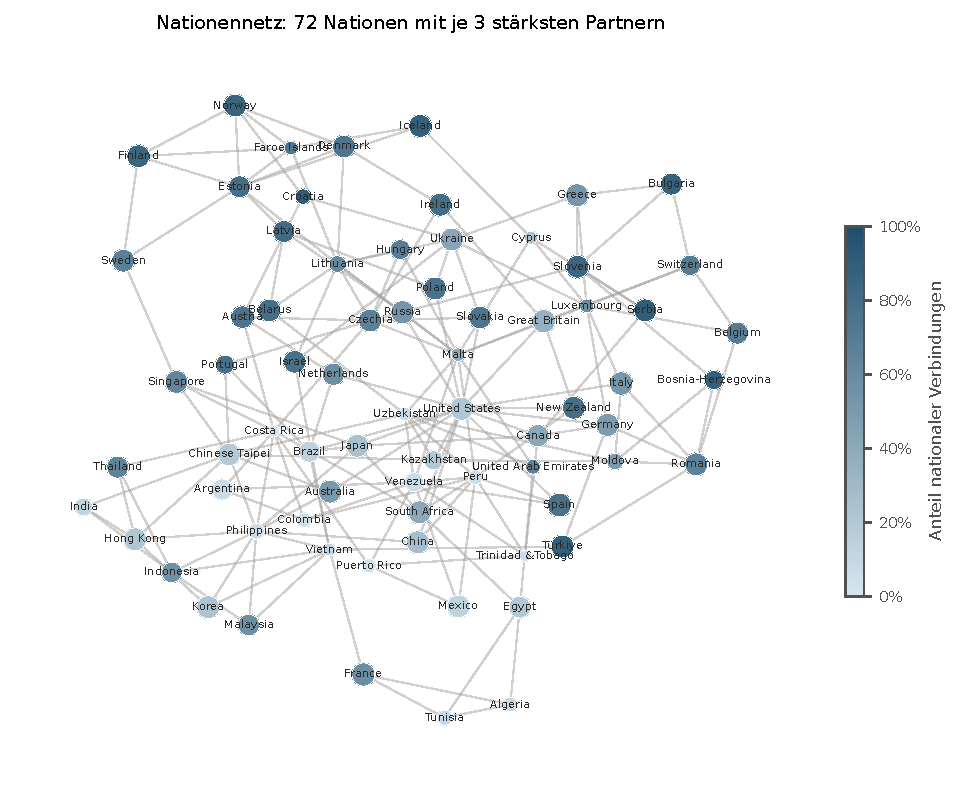
\includegraphics[width=0.8\textwidth]{04_nationennetz.pdf}
  \caption{Nationennetz der 72 Nationen mit mindestens 50 Athleten.
  Knotengrösse: Zahl der Athleten. Farbe: Anteil der Tage mit Landsleuten.
  Jede Nation ist mit ihren drei stärksten Partnern verbunden (gemeinsame
  Tage pro Athlet der Partnernation). Eigene Darstellung.}
  \label{fig:nationennetz}
\end{figure}

Trotz dieser internationalen Vernetzung verbinden 43,1\,\% der Kanten
Athleten derselben Nation, zusammen 53,1\,\% des Gesamtgewichts. Derselbe
Hypothesentest wie für das Geschlecht, nun mit permutierter Profilnation,
erwartet nur 1,2\,\%. Keine der 10\,000 Permutationen erreicht mehr als
1,3\,\%. Die nationale Prägung ist damit signifikant ($p < 0{,}0001$) und
mit $r = 0{,}25$ deutlich stärker als beim Geschlecht. Das passt zu
nationalen Meisterschaften, an denen vor allem Landsleute starten.
Abbildung~\ref{fig:nationen} vergleicht, welchen Anteil ihrer gemeinsamen
Tage die Athleten einer Nation mit Landsleuten teilen. Berücksichtigt sind
die 22 Nationen mit mindestens 200 Athleten, die damit ähnlich gross sind.
In Serbien, der Türkei, Slowenien und Finnland sind es über 80\,\%, in den
USA, Hongkong, Korea, Japan und China nur 21 bis 27\,\%. Diese Nationen sind
in den Listen vermutlich vor allem mit international startenden Athleten
vertreten.

\begin{figure}[H]
  \centering
  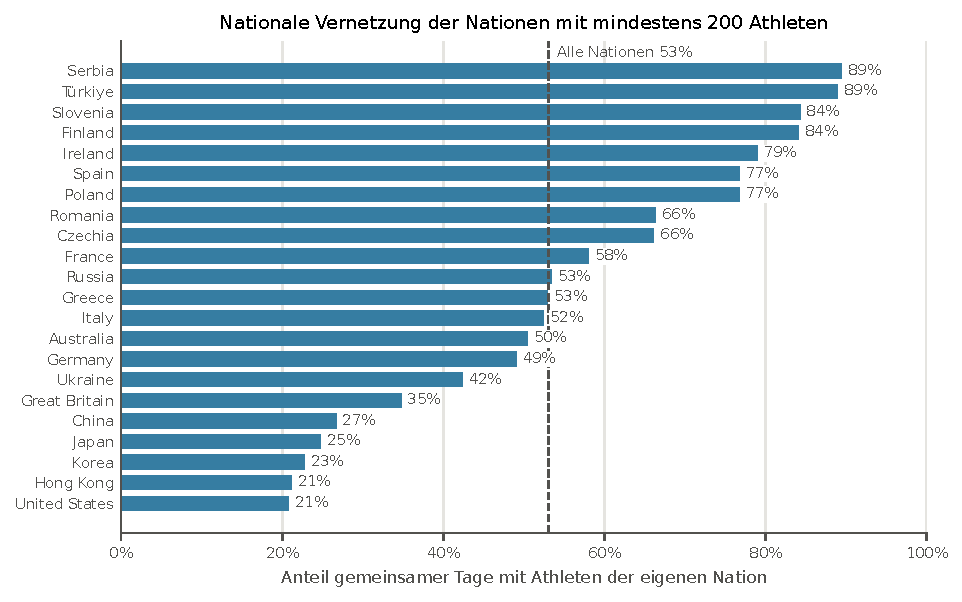
\includegraphics[width=0.85\textwidth]{04_nationen_intern.pdf}
  \caption{Anteil der gemeinsamen Tage mit Landsleuten für die 22
  Nationen mit mindestens 200 Athleten. Gestrichelt: Anteil über alle
  Nationen. Eigene Auswertung.}
  \label{fig:nationen}
\end{figure}

\subsection{Contextual View für die Schweiz}
Die Contextual View kombiniert beide Sichten. Die 160 Schweizer Athleten
bleiben einzelne Knoten (Local View), alle übrigen Athleten des
Arbeitsnetzes werden nach Nation zusammengefasst (Global View). Insgesamt
teilen die Schweizer 70\,\% ihrer gemeinsamen Tage mit Landsleuten, im
Median pro Athlet sogar 82\,\%. 152 von ihnen sind mit dem Ausland
verbunden, im Median mit Athleten aus sieben Nationen (mittlere 50\,\%
zwischen 4 und 15). Einzelne Athleten der internationalen Spitze verbinden die Schweiz
dagegen mit fast hundert Nationen, Noè Ponti mit 97 und Alexandre Haldemann
mit 89.

Abbildung~\ref{fig:contextual} zeigt diesen Unterschied für die 15
Schweizer mit den meisten gemeinsamen Tagen. Die oberen Athleten sind breit
mit dem Ausland verbunden, vor allem mit den vielen Nationen unter
\enquote{Übrige Nationen}, auf die 71\,\% aller Auslandstage der Schweizer
entfallen. Die unteren teilen ihre Tage überwiegend mit Landsleuten. Die internationale Einbindung der Schweiz hängt damit an
wenigen Personen. Wichtigster ausländischer Partner ist Liechtenstein,
dessen Athleten vermutlich regelmässig an Schweizer Wettkämpfen starten.

\begin{figure}[H]
  \centering
  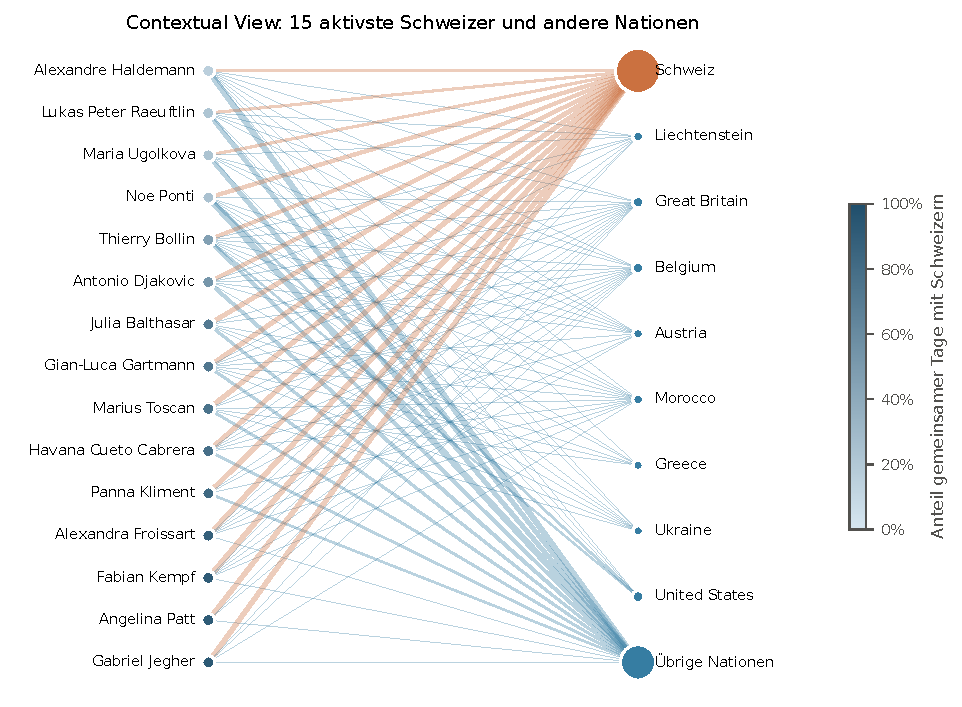
\includegraphics[width=0.9\textwidth]{04_contextual_schweiz.pdf}
  \caption{Contextual View für die 15 Schweizer mit den meisten
  gemeinsamen Tagen, sortiert von international (oben) zu national (unten).
  Farbe: Anteil der Tage mit Landsleuten. Rechts ihre Partner nach Nation
  zusammengefasst, die Kreisgrösse zeigt deren gemeinsame Tage mit den
  gezeigten Athleten. Linienstärke: gemeinsame Tage, orange mit Schweizern,
  blau mit dem Ausland. Eigene Darstellung.}
  \label{fig:contextual}
\end{figure}

\subsection{Ego-Netzwerk von Michael Phelps}
Als Ego wählen wir Michael Phelps, den Schwimmer mit den meisten
Olympiamedaillen. Im vollständigen Graphen hat er 708 Nachbarn, im Arbeitsnetz
bleiben 168 (Abbildung~\ref{fig:ego}). Nur 17\,\% davon stammen aus den USA,
insgesamt sind 61 Nationen vertreten. Die mittleren 50\,\% der Nachbarn sind
zwischen 1984 und 1990 geboren. Die meisten Verbindungen entstehen an der
Weltmeisterschaft 2009 in Rom (121 Nachbarn) und den Olympischen Spielen
2008 in Peking (51). Das passt zum lokalen Anstieg 2009 in
Abbildung~\ref{fig:eda}. Die stärksten Verbindungen mit vier oder fünf
gemeinsamen Tagen bestehen zu Allison Schmitt, Julia Smit, Peter Vanderkaay
und Darian Townsend.

\begin{figure}[H]
  \centering
  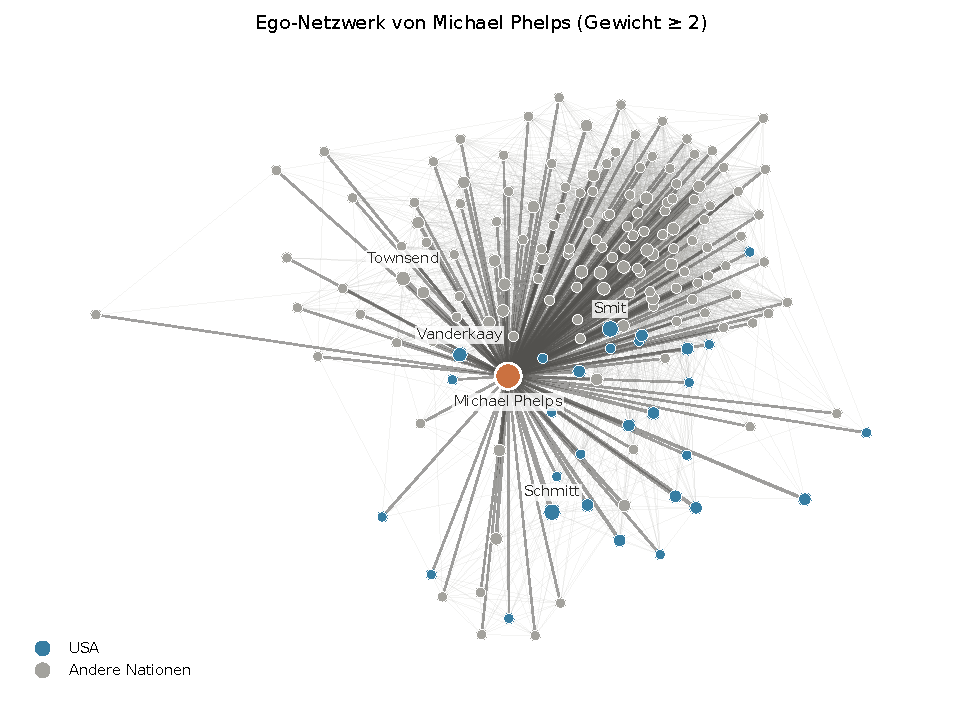
\includegraphics[width=0.85\textwidth]{04_ego_phelps.pdf}
  \caption{Ego-Netzwerk von Michael Phelps (orange) mit 168 Nachbarn,
  blau aus den USA, grau aus anderen Nationen. Knotengrösse und dunkle Linien
  zeigen die gemeinsamen Tage mit Phelps, beschriftet sind Nachbarn ab vier
  Tagen. Hellgraue Linien verbinden Nachbarn untereinander. Eigene
  Darstellung.}
  \label{fig:ego}
\end{figure}

Unter den Nachbarn beträgt die Density 0,26, im gesamten Arbeitsnetz nur
0,0041. Diese Dichte entsteht durch die Modellierung, denn jeder
Veranstaltungstag verbindet alle dort erfassten Athleten. Das
Ego-Netzwerk zeigt somit vor allem die Veranstaltungen, an denen Phelps
seine Bestleistungen erzielte, und keine persönlichen Kontakte.
